\chapter{Strong Coupling and the Migdal Kadanoff Ladder}\label{ch:strong}

We now move to four dimensions. Chapter~\ref{ch:twod} ended with the models that can be solved exactly, where the heat kernel and the transfer matrix gave the gap at every coupling. In four dimensions nothing is exact. This chapter treats the end of the coupling range where everything is under control, strong coupling, and explains why control there does not reach the continuum. It then describes how glueball masses are measured by lattice Monte Carlo, introduces the Migdal Kadanoff ladder, a renormalization group that can be followed from weak to strong coupling at the price of an approximation, and records what was computed on it, with the arithmetic stated. The gap between the two ends of the coupling range is the subject of the remaining chapters.

\section{Strong Coupling and the Lattice}\label{sec:strongc}

\subsection{The character expansion}

For SU(2) with the Wilson action\index{Wilson action}\cite{Wi74}, each plaquette carries the weight $e^{\beta\cos\theta_p}$, where $\theta_p$ is the rotation angle of the plaquette holonomy. Expand it in characters:
\[
e^{\beta\cos\theta}=I_1(\beta)\cdot\frac{2}{\beta}\Big(1+\sum_{n\ge2}n\,u_n(\beta)\,\chi_n(\theta)\Big),\qquad u_n=\frac{I_n(\beta)}{I_1(\beta)} .
\]
At strong coupling, $\beta\to0$, the coefficients are small: $u_n(\beta)\sim(\beta/2)^{n-1}/n!$, and in particular $u_2\sim\beta/4$. The partition function becomes a sum over assignments of representations to plaquettes, and orthogonality of characters under the Haar integrals over links forces the nonzero assignments to form closed surfaces. Each surface of $|P|$ plaquettes in the fundamental representation contributes a factor of order $u_2^{|P|}$.

\subsection{The Osterwalder and Seiler theorem}

Osterwalder and Seiler\index{Osterwalder, K.!and Seiler, E.}\cite{OSe} turned this surface expansion into a convergent cluster expansion\index{cluster expansion}.

\begin{theorem}[Osterwalder and Seiler \cite{OSe}]
For four dimensional lattice gauge theory with the Wilson action and compact gauge group, there is $\beta_0>0$ such that for $\beta<\beta_0$ the infinite volume limit exists, is unique, satisfies reflection positivity\index{reflection positivity}, and has exponential clustering for gauge invariant observables at some positive rate. The best such rate, the lattice mass $m(\beta)>0$, grows like $|\log\beta|$ as $\beta\to0$, and Wilson loop\index{Wilson loop}s obey an area law.
\end{theorem}

The leading behaviour of the mass can be read off from the smallest surfaces that connect two plaquette observables separated by $\tau$ lattice steps in time: a tube whose cross section is the plaquette itself, made of four plaquettes per time step. M\"unster and others computed the series~\cite{Mu81b}, whose leading term is
\[
m(\beta)=-4\log u_2(\beta)+O(u_2).
\]
For SU(2) this gives the following values.
\begin{center}
\begin{tabular}{rcc}
\toprule
$\beta$ & $u_2(\beta)$ & $-4\log u_2(\beta)$ \\ \midrule
0.1 & 0.0250 & 14.76 \\
0.5 & 0.1237 & 8.36 \\
1.0 & 0.2402 & 5.71 \\
1.5 & 0.3441 & 4.27 \\
2.0 & 0.4331 & 3.35 \\
\bottomrule
\end{tabular}
\end{center}
The leading term is reliable only well inside the convergence region, but it shows the scale: at strong coupling the glueball\index{glueball} mass is several inverse lattice spacings, and its correlation length is a fraction of a lattice spacing.

\subsection{The Thorin gap inequality in lattice units}

The theorem can be combined with the equivalence theorem of Section~\ref{ch:routeB}, but only with two further steps that we have not taken.

\begin{remark}
For $\beta<\beta_0$ the infinite volume theory clusters at the rate $m(\beta)$, which points to the uniform Thorin gap inequality in lattice units with $K=1$ and $\Delta_0=m(\beta)$. The theorem as stated gives clustering only for the infinite volume limit, so uniformity in the volume does not follow from it. Theorem~\ref{thm:equivB} also needs the supremum over $a$ of $\int e^{-\alpha_0E}\,d\mu^{(a)}$ to be finite, and we have not checked this. We use the statement only as a guide to the shape of the Thorin density at strong coupling.
\end{remark}

At strong coupling we expect, heuristically, the spectral measure\index{spectral measure}s to be dominated by a single atom at $m(\beta)$, with weight $w$, so the Route B Thorin density\index{Thorin density} is approximately
\[
T_\alpha(z)\approx\frac{w}{\pi\kappa}\,e^{-\alpha m(\beta)}\big(1-\cos \kappa\,m(\beta)\big),\qquad \kappa=\sqrt{2z},
\]
a single oscillation in real time, damped in Euclidean time at the lattice mass.

\subsection{Why strong coupling does not reach the continuum}

The continuum limit is the opposite end of the coupling range. Asymptotic freedom\cite{GW73,Po73} fixes how the lattice spacing must shrink as $\beta$ grows. For SU(2) at one loop,
\[
a(\beta)\,\Lambda\propto\exp\Big(-\frac{3\pi^2}{11}\beta\Big),
\]
with a two loop correction that multiplies the right side by a power of $\beta$. A physical gap requires the lattice mass to shrink at the same rate:
\[
\Delta_{\mathrm{phys}}=\frac{m(\beta)}{a(\beta)}\quad\text{bounded below as }\beta\to\infty .
\]
Figure~\ref{fig:strongscaling} shows the two regimes on one plot. The strong coupling mass decreases slowly, like $\log(1/\beta)$. The scaling form decreases exponentially in $\beta$. Lattice Monte Carlo\cite{Cr80,Te98} shows that for SU(2) the true lattice mass crosses smoothly from the first to the second, with no phase transition, around $\beta\approx2$. The cluster expansion is only known to converge for $\beta<\beta_0$. No expansion known to us controls $m(\beta)$ uniformly across it.

\begin{figure}[t]
\centering
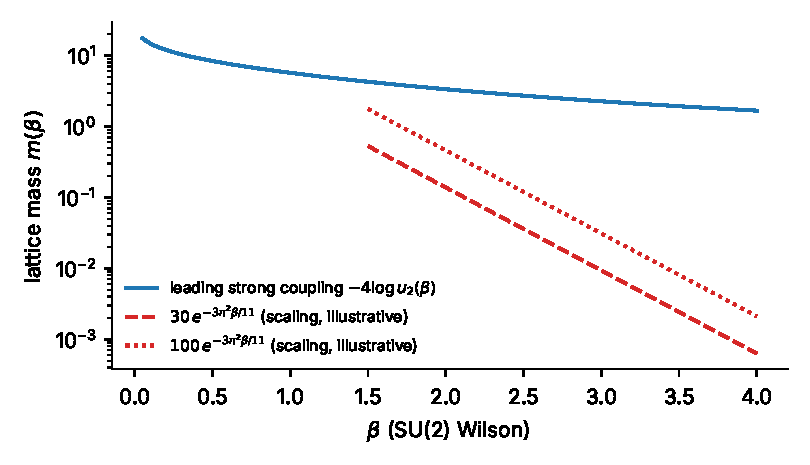
\includegraphics[width=0.92\textwidth]{figures/strong_vs_scaling.pdf}
\caption[The two ends of the coupling range for SU(2)]{The two ends of the coupling range for SU(2). The leading strong coupling mass $-4\log u_2(\beta)$ is controlled by the cluster expansion for small $\beta$. The continuum limit requires the scaling behaviour $m(\beta)\propto e^{-3\pi^2\beta/11}$ as $\beta\to\infty$; the prefactors shown are illustrative. The mass gap problem lives in the crossover between them.}
\label{fig:strongscaling}
\end{figure}

\subsection{What would bridge the gap}

The two dimensional proof of Chapter~\ref{ch:twod} suggests the shape of what is needed. There, an explicit transfer matrix\index{transfer matrix} eigenvalue was bounded at every coupling by a special function inequality whose weak coupling behaviour exactly matched the conversion to physical units. In four dimensions we would like a lower bound
\[
m(\beta)\ge f(\beta)\quad\text{for all }\beta,\qquad\liminf_{\beta\to\infty}\frac{f(\beta)}{a(\beta)}>0 .
\]
We call this a transfer matrix Bessel inequality. Strong coupling supplies it for $\beta<\beta_0$, and asymptotic freedom\index{asymptotic freedom} says what $f$ must look like for large $\beta$. The difficulty is everything in between.

Renormalization group methods are the classical tool for crossing scales. Ba\l aban\index{Balaban, T.@Ba\l aban, T.}'s rigorous renormalization group for lattice gauge theory\cite{Ba87} controls the theory at weak coupling, at short distances, and in the later papers of the series proves ultraviolet stability. What it does not do is follow the flow into the strong coupling regime at long distances, where the gap is generated. Section~\ref{ch:mk} studies a renormalization group that can be followed all the way, at the price of an approximation, and reads it through the probabilistic toolkit.

\section{Lattice Monte Carlo for Glueballs}\label{ch:latticemc}\index{glueball}\index{heat bath}\index{overrelaxation}\index{smearing}

The predictions of the Migdal Kadanoff ladder, and the gap estimator of Chapter~\ref{ch:estimation}, both need lattice data at intermediate and weak coupling. This section describes how glueball correlators are measured in four dimensions and where the statistical difficulties lie.

\subsection{Updates}

For SU(2) the standard update is the heat bath of Creutz\cite{Cr80}, in the Kennedy and Pendleton form\cite{KP85} at weak coupling, which samples each link exactly from its von Mises Fisher conditional (Section~\ref{ch:latent}). For SU(3) the Cabibbo and Marinari~\cite{CM82} method applies the SU(2) heat bath to a sequence of SU(2) subgroups. Overrelaxation reflects each link through the direction of its staple sum, leaving the action unchanged; it is microcanonical and must be combined with heat bath steps, but it reduces autocorrelations substantially. Hybrid Monte Carlo~\cite{DKPR87} moves all links together along Hamiltonian trajectories and is the method of choice when fermions are present; for pure gauge theory the heat bath and overrelaxation combination remains very efficient.

Figure~\ref{fig:plaqhist} shows the output of our own four dimensional heat bath, used in Chapter~\ref{ch:progress}: plaquette histories on an $8^4$ lattice at five couplings, and their autocorrelations, which die out within a few sweeps. The plaquette is the easiest observable; glueball correlators, discussed next, are far noisier.

\begin{figure}[t]
\centering
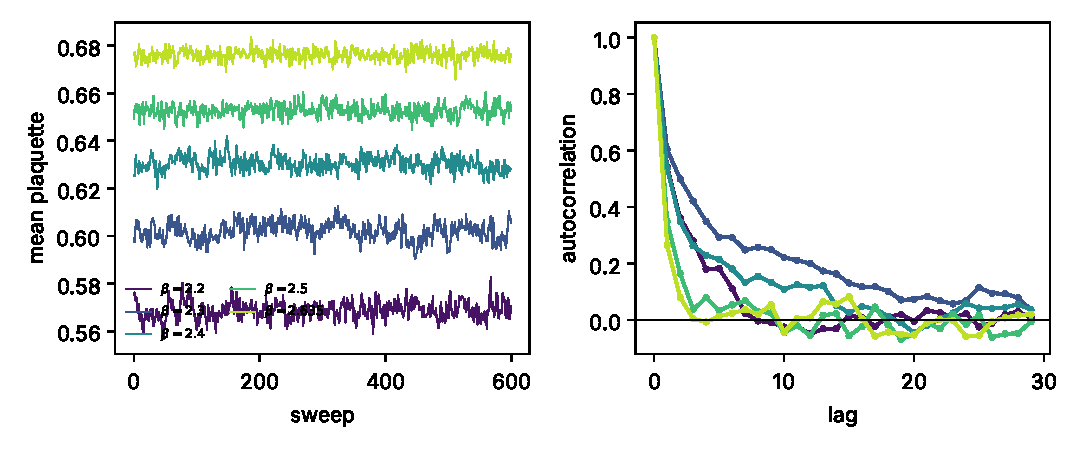
\includegraphics[width=0.95\textwidth]{figures/plaquette_history.pdf}
\caption[Four dimensional SU(2) plaquette histories]{Mean plaquette histories over six hundred heat bath sweeps on an $8^4$ lattice at five couplings (left) and their autocorrelation functions (right).}
\label{fig:plaqhist}
\end{figure}

\subsection{Glueball operators}

A glueball operator is a gauge invariant combination of Wilson loops at a fixed time, summed over space to project onto zero momentum, with the combination chosen to transform in an irreducible representation of the cubic group and of parity and charge conjugation. The scalar $0^{++}$ uses sums of plaquettes; the tensor $2^{++}$ uses differences of plaquette orientations. Because the lightest glueball mass in lattice units is of order one or below at accessible couplings, its correlator falls below the noise within a few time slices. Three techniques are essential.
\begin{itemize}
\item Smearing replaces each spatial link by an average over paths, as in APE~\cite{APE87} or stout smearing~\cite{MP04}, so that operators are extended objects with better overlap on the ground state.
\item Variational analysis builds a matrix of correlators $C_{ij}(\tau)$ from many operators and solves the generalised eigenvalue problem $C(\tau)v=\lambda(\tau,\tau_0)C(\tau_0)v$. The eigenvalues decay with the masses of the lowest states, separating them. In the language of this book, this is a matrix version of the spectral measure, and its positivity is reflection positivity of the matrix valued correlator.
\item Anisotropic lattices use a finer spacing in time than in space, giving more time slices before the signal is lost, as in Morningstar and Peardon's\cite{MP} glueball spectrum.
\end{itemize}

\subsection{The signal to noise problem}

The variance of a glueball correlator does not decay with $\tau$, because $|O|^2$ has a vacuum expectation value, while the signal decays like $e^{-m\tau}$. The signal to noise ratio therefore falls exponentially. L\"uscher and Weisz\cite{LW01} introduced multilevel algorithms, which exploit the locality of the action to average sub lattices independently with the boundary fixed, reducing the variance exponentially in the number of levels.

\subsection{Topological freezing and open boundaries}

At fine lattice spacing the topological charge freezes, as shown for two dimensional U(1) in Figure~\ref{fig:u1}. Schaefer, Sommer and Virotta~\cite{SSV11} showed the effect in four dimensional SU(3) and its influence on other observables. L\"uscher and Schaefer~\cite{LS11} proposed open boundary conditions in time, which let topological charge flow in and out of the lattice and remove the barrier. Other remedies include parallel tempering in boundary conditions and density of states methods\cite{LLR}; split sampling by topological sector (Section~\ref{ch:vertical}) is a candidate that we have not tested.

\subsection{From data to the gap}

The output of a glueball computation is a set of correlators at a few couplings, each with an estimated lattice mass and its uncertainty, typically with autocorrelations estimated by the Madras and Sokal\cite{MS88} windowing of Section~\ref{ch:sokal}. Chapter~\ref{ch:estimation} proposed estimating the gap as a support constraint on a positive measure, and noted that local rates and the profile estimate err toward a larger gap, so that data bound the true gap from above. The Migdal Kadanoff ladder predicts the lattice mass as a function of the coupling, through the number of steps to strong coupling. Comparing that prediction with published lattice masses\cite{MP,Te98} is a test of the caricature, and therefore of the plausibility of the comparison step on which the path of Chapter~\ref{ch:path} depends.

\section{The Migdal Kadanoff Ladder}\label{ch:mk}

In 1975 Migdal\cite{Mi75} proposed a renormalization group for lattice gauge theories that is simple enough to iterate to arbitrarily long distances. Kadanoff\cite{Ka75,Ka76} explained it as a combination of two moves on the lattice, and showed that one of them is exact in two dimensions and the other gives one sided bounds. This section reads the recursion probabilistically: it alternates a Bayesian product of likelihoods with a convolution of laws on the group. Flat space would make the coupling marginal in four dimensions. The curvature of the group makes it run, and the size of the effect is the mean of the Biane Pitman Yor\index{Biane Pitman Yor variable}\cite{BPY} variable $S_{\mathrm{BPY}}$.

\subsection{Bond moving and decimation}

Consider a hypercubic lattice in $d$ dimensions and a scale factor $b\ge2$. One Migdal Kadanoff\index{Migdal Kadanoff recursion} step does two things to every plaquette weight $f$.
\begin{enumerate}
\item[(i)] Bond moving. In each plane, the plaquettes in a $b\times b$ block are moved, in the $d-2$ transverse directions, onto a single plane, so each surviving plaquette carries $k=b^{d-2}$ copies of the original weight: $f\mapsto f^{\,k}$.
\item[(ii)] Decimation. In that plane, the $b\times b$ block of strengthened plaquettes is glued into one by integrating out the interior links. As in two dimensions, this is a convolution of class functions, and in character variables $u_n\mapsto u_n^{\,b^2}$.
\end{enumerate}
After the step the lattice spacing is $ba$. On the hierarchical lattice built by iterating these two moves, the recursion is exact. On $\Z^d$ it is an approximation, and bond moving\index{bond moving} is where the approximation enters. Kadanoff showed that moving bonds in one direction raises, and in the other lowers, the free energy, which gives one sided bounds that we discuss in Chapters~\ref{ch:path} and~\ref{ch:sandwich}.

\subsection{A probabilistic reading}

Normalise the plaquette weight to a probability density $f$ with respect to Haar measure\index{Haar measure} on SU(2). Then:
\begin{itemize}
\item Bond moving replaces $f$ by $f^k/\int f^k$. This is the posterior obtained by combining $k$ independent copies of the likelihood $f$ for an unknown group element, starting from the flat Haar prior. It is a Bayesian product.
\item Decimation replaces $f$ by the $b^2$ fold convolution $f^{*b^2}$. This is the law of a product of $b^2$ independent random group elements with law $f$. For Brownian laws it adds times.
\end{itemize}
So one step of the renormalization group is a product followed by a convolution. In the language of Polson and Scott's\cite{PSdual} duality between envelopes and mixtures, bond moving is an envelope and decimation\index{decimation} is a mixture.

\begin{lemma}[positivity is preserved]\label{lem:posB}
If $f$ has nonnegative character coefficients, so does its image under one Migdal Kadanoff step.
\end{lemma}

\begin{proof}
Decimation raises the coefficients to the power $b^2$. For bond moving, the Clebsch Gordan\index{Clebsch Gordan rule} rule for SU(2),
\[
\chi_p\chi_n=\sum_{j=|p-n|+1,\ \text{step }2}^{p+n-1}\chi_j,
\]
has every multiplicity equal to one, hence nonnegative. So products of class functions with nonnegative coefficients have nonnegative coefficients, and so do powers. For general compact groups the same holds because tensor product multiplicities are nonnegative integers.
\end{proof}

By the Bochner theorem of Chapter~\ref{ch:positivity} (Proposition~\ref{prop:bochnergroup}), nonnegative coefficients are positive definiteness, which is the Osterwalder Seiler condition for reflection positivity\index{reflection positivity}. Every rung of the ladder is therefore the $\Z^4$ lattice theory with that plaquette weight, which is reflection positive with genuine nonnegative spectral measure\index{spectral measure}s, and the tools of Sections~\ref{ch:routeA} and~\ref{ch:routeB} apply at each rung.

\subsection{The Gaussian ledger}

At weak coupling the plaquette law is concentrated near the identity, where the group looks like its Lie algebra $\R^3$. Suppose for a moment that the law were exactly Gaussian on $\R^3$ with precision $\rho$ per coordinate. Then the two operations act by simple arithmetic:
\[
\text{bond moving: }\rho\mapsto k\rho,\qquad\text{decimation: }\rho\mapsto \rho/b^2 .
\]
With $k=b^{d-2}$ the net effect is $\rho\mapsto b^{d-4}\rho$. In two dimensions the precision falls by $b^2$ per step, which is the exact decimation of Chapter~\ref{ch:twod}. In three dimensions it falls by $b$. In four dimensions it is unchanged: the coupling is marginal. Whatever makes the four dimensional coupling run must come from the departure of the group from flat space.

\subsection{Curvature and the Biane Pitman Yor variable}

The departure is visible in the small time form of the heat kernel\index{heat kernel} from Chapter~\ref{ch:twod},
\[
K_t(\theta)\approx C\,t^{-3/2}\,\frac{\theta}{\sin\theta}\,e^{-\theta^2/t}.
\]
The Gaussian part has precision proportional to $1/t$; the factor $\theta/\sin\theta$ is the curvature correction. Raising to the power $k$,
\[
K_t^k\propto\Big(\frac{\theta}{\sin\theta}\Big)^{k-1}\cdot\frac{\theta}{\sin\theta}\,e^{-k\theta^2/t}\propto\Big(\frac{\theta}{\sin\theta}\Big)^{k-1}K_{t/k}(\theta).
\]
The extra factor $(\theta/\sin\theta)^{k-1}$ is the whole of the correction. Continue it to imaginary angle, $\theta=ix$:
\[
\Big(\frac{x}{\sinh x}\Big)^{k-1}=\E\exp\Big(-\frac{x^2}{2}\sum_{j=1}^{k-1}S_{\mathrm{BPY},j}\Big),
\]
where the $S_{\mathrm{BPY},j}$ are independent copies of the Biane Pitman Yor variable with Laplace transform $\sqrt{2\lambda}/\sinh\sqrt{2\lambda}$. To second order in $x$ this is $\exp(-(k-1)\E S_{\mathrm{BPY}}\,x^2/2)$, and returning to real angle the curvature factor is a Gaussian tilt $\exp((k-1)\E S_{\mathrm{BPY}}\,\theta^2/2)$ that removes precision.

\begin{figure}[t]
\centering
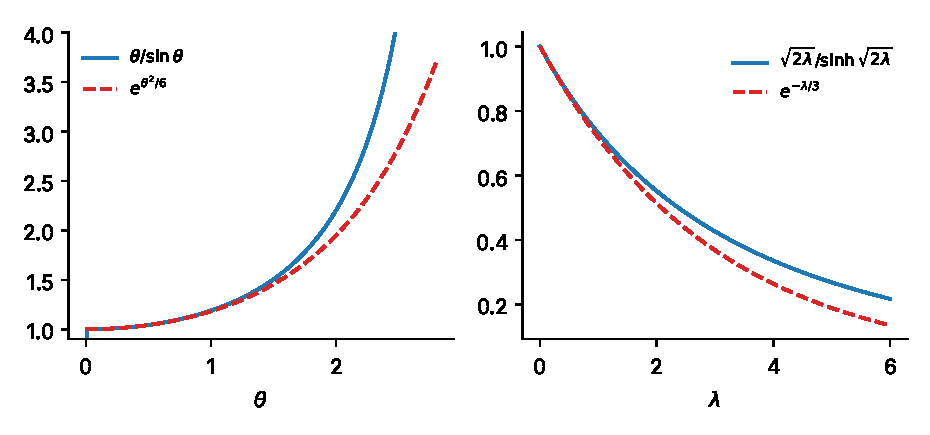
\includegraphics[width=\textwidth]{figures/curvature_bpy.pdf}
\caption[Left: the curvature factor $\theta/\sin\theta$ and its Gaussian approximation $e^{\theta^2/6}$]{Left: the curvature factor $\theta/\sin\theta$ and its Gaussian approximation $e^{\theta^2/6}$. Right: at imaginary angle the same factor is the Laplace transform $\sqrt{2\lambda}/\sinh\sqrt{2\lambda}$ of the Biane Pitman Yor variable $S_{\mathrm{BPY}}$, compared with $e^{-\lambda\E S_{\mathrm{BPY}}}=e^{-\lambda/3}$.}
\label{fig:curvatureB}
\end{figure}

\begin{remark}[leading order derivation: the decrement]\label{prop:decrementB}
For the heat kernel action with small $t=2/\beta$, one Migdal Kadanoff step with scale $b$ in dimension $d$ maps $t$ to $t''$ with
\[
\frac1{t''}=\frac{b^{d-4}}{t}-\frac{(b^{d-2}-1)\,\E S_{\mathrm{BPY}}}{2b^2}+O(t).
\]
In four dimensions,
\[
\beta''=\beta-\big(1-b^{-2}\big)\E S_{\mathrm{BPY}}+O(1/\beta)=\beta-\frac{b^2-1}{3b^2}+O(1/\beta).
\]
This is a leading order derivation: the Gaussian approximation of $\theta/\sin\theta$ is made without bounding the $O(t)$ and $O(1/\beta)$ remainders, so the remainders are not proved to be of that order.
\end{remark}

\begin{proof}[Derivation]
Write the heat kernel near the identity as a Gaussian of precision $2/t$ in $\theta$, times the curvature factor. Bond moving multiplies the Gaussian precision by $k$ and multiplies the law by $(\theta/\sin\theta)^{k-1}\approx e^{(k-1)\E S_{\mathrm{BPY}}\,\theta^2/2}$, so the new precision is $2k/t-(k-1)\E S_{\mathrm{BPY}}$, that is $1/t'=k/t-(k-1)\E S_{\mathrm{BPY}}/2$. Decimation divides the precision by $b^2$. With $k=b^{d-2}$ this gives the first formula, and with $d=4$ and $\beta=2/t$ the second.
\end{proof}

At $b=2$ the decrement is $\frac34\cdot\frac13=\frac14$; at $b=3$ it is $\frac89\cdot\frac13=\frac{8}{27}$. The one loop decrement for SU(2), from Chapter~\ref{ch:problem}, is $\frac{11\ln b}{3\pi^2}$ in units of $\beta$ per step, which is $0.2575$ at $b=2$ and $0.408$ at $b=3$. So at $b=2$ the Migdal Kadanoff coefficient is within three percent of the one loop value. That agreement is specific to $b=2$: as $b\to1$ the Migdal Kadanoff rate per unit $\log b$ tends to $2/3$, against the true $0.3715$. The recursion is a scheme, not an exact computation.

\subsection{SU(N)}

For SU(N) with Wilson weight $\exp(\frac\beta N\operatorname{Re}\operatorname{tr}U)$, write the eigenvalues of a group element as $e^{i\theta_1},\dots,e^{i\theta_N}$ with $\sum\theta_i=0$. Near the identity the Wilson weight is approximately $\exp(-\frac{\beta}{2N}\sum\theta_i^2)$. The Jacobian of the exponential map is a product over positive roots,
\[
j(\theta)^{-1/2}=\prod_{i<j}\frac{(\theta_i-\theta_j)/2}{\sin\big((\theta_i-\theta_j)/2\big)},
\]
so the curvature factor is a product of $N(N-1)/2$ Biane Pitman Yor factors. Using
\[
\sum_{i<j}(\theta_i-\theta_j)^2=N\sum_i\theta_i^2\qquad\text{when }\sum_i\theta_i=0,
\]
the tilt is isotropic and the Gaussian ledger closes exactly as for SU(2).

\begin{remark}[leading order derivation: the SU(N) decrement]\label{prop:sunB}
At weak coupling one Migdal Kadanoff step in four dimensions gives
\[
\beta''=\beta-\big(1-b^{-2}\big)\frac{N^2}{4}\,\E S_{\mathrm{BPY}}+O(1/\beta)=\beta-\big(1-b^{-2}\big)\frac{N^2}{12}+O(1/\beta).
\]
The one loop decrement is $\frac{11N^2\ln b}{12\pi^2}$, so the ratio of the two is $\frac{\pi^2(1-b^{-2})}{11\ln b}$, independent of $N$. At $b=2$ it equals $\frac{12\pi^2}{176\ln2}=0.971$. As for the SU(2) case, the remainder is not bounded.
\end{remark}

\begin{proof}[Derivation]
In terms of $c=\beta/N$, the Gaussian precision per coordinate $\theta_i$ is $c$. Bond moving gives $kc$ minus the tilt $(k-1)\E S_{\mathrm{BPY}}\cdot\frac14\cdot N$, from $\sum_{i<j}\frac{(\theta_i-\theta_j)^2}{4}=\frac N4\sum\theta_i^2$. Decimation divides by $b^2$. With $k=b^2$ and $\beta=Nc$ the stated decrement follows, and for $N=2$ it reduces to Remark~\ref{prop:decrementB}.
\end{proof}

We checked Remark~\ref{prop:sunB} for SU(3) numerically, in double precision, with a full computation: class functions on the maximal torus, the Weyl character formula\index{Weyl character formula} on a $192\times192$ grid, $1081$ irreducible representations, and the coupling defined by matching the fundamental character coefficient to the Wilson action\index{Wilson action}. The decrement is $0.581$, $0.572$, $0.569$ and $0.568$ at $\beta=12,16,20,24$, approaching $9/16=0.5625$ at rate $1/\beta$ (Figure~\ref{fig:su3B}). The one loop value is $0.5794$.

\begin{figure}[t]
\centering
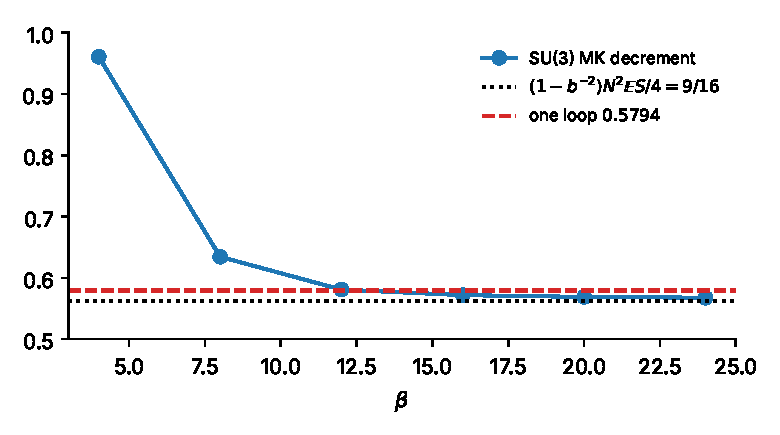
\includegraphics[width=0.9\textwidth]{figures/su3_decrement.pdf}
\caption[SU(3) Migdal Kadanoff decrement per step at $b=2$, from a full computation with Weyl characters]{SU(3) Migdal Kadanoff decrement per step at $b=2$, from a full computation with Weyl characters. It approaches the prediction $9/16$ of Remark~\ref{prop:sunB}, three percent below the one loop value.}
\label{fig:su3B}
\end{figure}

\subsection{The full flow for SU(2)}

We ran the recursion for SU(2) with $b=2$ and $d=4$, starting from the Wilson action, in double precision floating point, with class functions represented by up to $1500$ characters and $6000$ point Gauss Legendre quadrature. Apart from the proved Lemma~\ref{lem:mlrB} and Proposition~\ref{prop:criterionB}, this section and the next are numerical results: nothing else in them carries an enclosure or an interval bound. The code reproduces $I_n/I_1$ for $n=2,3$ at $\beta=3$ to double precision. Figure~\ref{fig:mklevelsB} follows the Thorin levels $u_n$ along a trajectory started at $\beta=6$. They stay close to one for about twenty steps while the coupling drifts down, then collapse together within a few steps as the flow enters strong coupling.

\begin{figure}[t]
\centering
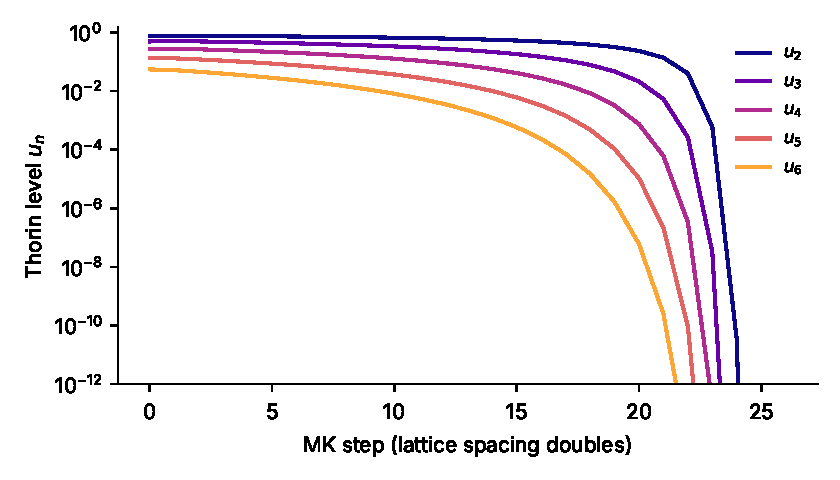
\includegraphics[width=0.9\textwidth]{figures/mk_levels.pdf}
\caption[Thorin levels $u_n$ along the SU(2) Migdal Kadanoff flow from the Wilson action at $\beta=6$]{Thorin levels $u_n$ along the SU(2) Migdal Kadanoff flow from the Wilson action at $\beta=6$. Each step doubles the lattice spacing. The slow drift followed by a sudden collapse is the logarithmic running of asymptotic freedom followed by the onset of confinement.}
\label{fig:mklevelsB}
\end{figure}

Defining the effective coupling $\beta_{\mathrm{eff}}$ by matching $u_2$ to the Wilson value, the flow has the following features (Figure~\ref{fig:mkflowB}).
\begin{itemize}
\item For initial $\beta\ge2$ the first step from the Wilson action raises $\beta_{\mathrm{eff}}$, by between $0.1$ and $0.37$. The Wilson action is not on the renormalized trajectory, and the first step appears to project onto it.
\item After the first step the decrement is positive along every trajectory and at every coupling sampled. It peaks at about $0.42$ near $\beta_{\mathrm{eff}}\approx0.8$, the crossover, and tends to $0.249+0.032/\beta$ at weak coupling.
\item Every initial coupling sampled reaches strong coupling. The number of doublings needed grows like $3.98\,\beta$, against $4$ from Remark~\ref{prop:decrementB} and $3.88$ from one loop asymptotic freedom.
\end{itemize}
\begin{center}
\begin{tabular}{rcc}
\toprule
initial $\beta$ & $\beta_{\mathrm{eff}}$ after one step & doublings to $u_2<0.02$ \\ \midrule
2 & 2.109 & 7 \\
4 & 4.305 & 15 \\
8 & 8.354 & 31 \\
16 & 16.366 & 63 \\
24 & 24.370 & 94 \\
\bottomrule
\end{tabular}
\end{center}


\begin{figure}[t]
\centering
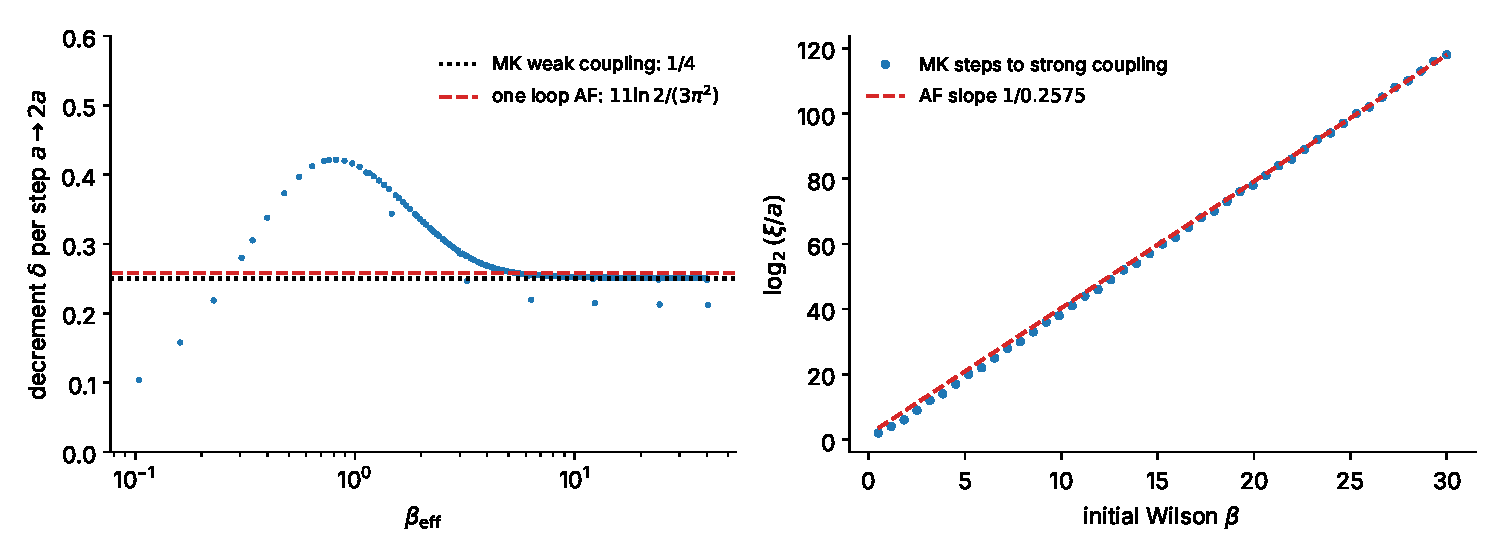
\includegraphics[width=\textwidth]{figures/mk_flow.pdf}
\caption[SU(2) Migdal Kadanoff flow from the Wilson action]{SU(2) Migdal Kadanoff flow from the Wilson action. Left: the decrement per step along six trajectories. Right: the number of doublings to strong coupling is linear in $\beta$, with a slope close to the one loop value of asymptotic freedom.}
\label{fig:mkflowB}
\end{figure}

In the computed flows there is no fixed point at finite coupling, and every coupling flows to confinement\index{confinement}. This is Migdal's original observation, and on the hierarchical lattice where the recursion is exact, Ito\index{Ito, K. R.}\cite{Ito85} proved confinement at all couplings in 1985. What the probabilistic reading adds is an explanation of the rate, through a single number, the mean of a generalized gamma convolution\index{generalized gamma convolution}\cite{Bo92}, together with the positivity of every rung. Section~\ref{ch:verification} sets the numerical observation that the decrement is positive beside a one dimensional map and a proved inequality.

\section{Checking the Ladder}\label{ch:verification}

Section~\ref{ch:mk} observed that the Migdal Kadanoff\index{Migdal Kadanoff recursion} coupling decreases at every step. This section states the observation for an explicit one dimensional map and records exactly what was computed, proves the monotonicity that the check needs from a likelihood ratio\index{likelihood ratio order} property of the heat kernel\index{heat kernel}, and reads the correlation length as a first passage time\index{first passage time}.

\subsection{The heat kernel projected map}

The full recursion acts on an infinite sequence of character coefficients. To obtain a one dimensional map we project onto the heat kernel family after each step.

\begin{definition}
For $\beta>0$ let $t=2/\beta$ and start from the heat kernel law $u_n=e^{-t(n^2-1)/4}$. Apply one Migdal Kadanoff step with $b=2$ and $d=4$, read off the new second coefficient $u_2''$, and define $R(\beta)=2/t''$ where $u_2''=e^{-3t''/4}$.
\end{definition}

Starting from the heat kernel removes the first step anomaly of the Wilson action\index{Wilson action}. The projection is a definition, and the exact recursion acts on all character coefficients. The following checks, all in double precision, test the projection and the map numerically.
\begin{itemize}
\item Reducing the number of characters from $1500$ to $800$ and the number of quadrature points from $6000$ to $4000$ changes $R$ by less than $10^{-11}$ on the tested points.
\item Iterating $R$ reproduces the unprojected flow, started from the same heat kernel law, to within $0.012$ over eight steps from $\beta=3$, and to within $0.003$ from $\beta=10$.
\item At $b=3$ (the same projection with $b=3$) the decrement $\beta-R(\beta)$ is $0.2974$, $0.2969$ and $0.2966$ at $\beta=10,20,40$, approaching $8/27=0.2963$ as Remark~\ref{prop:decrementB} predicts.
\end{itemize}
At $b=2$ the decrement is $0.2726$ at $\beta=0.5$, $0.2806$ at $\beta=1$, $0.2623$ at $\beta=2$, $0.2544$ at $\beta=5$, $0.2521$ at $\beta=10$ and $0.2504$ at $\beta=50$. Above $\beta=20$ it fits $0.25000+0.021/\beta$.

\subsection{Monotonicity from a likelihood ratio}

\begin{lemma}\label{lem:mlrB}
Suppose the SU(2) heat kernel has monotone likelihood ratio in time, meaning that $\partial_\theta\log K_t(\theta)$ is increasing in $t$ for every $\theta\in(0,\pi)$. Then $R$ is increasing.
\end{lemma}

\begin{proof}
After bond moving\index{bond moving}, the second normalised character coefficient is $u_2=\E_{\nu_t}[\cos\theta]$, where $\nu_t\propto K_t^k$ times the Haar density, because $\chi_2(\theta)/2=\cos\theta$. Monotone likelihood ratio passes from $K_t$ to $K_t^k$, since $\partial_\theta\log K_t^k=k\,\partial_\theta\log K_t$. By Proposition~\ref{prop:lro}(i) of Section~\ref{ch:toolkit}, $\nu_{t'}$ is then stochastically larger than $\nu_t$ for $t'>t$, so $\E_{\nu_t}\cos\theta$ is decreasing in $t$. Decimation $u\mapsto u^{b^2}$ and the conversion back to $\beta$ are increasing, and $t=2/\beta$ is decreasing in $\beta$. Composing, $R$ is increasing.
\end{proof}

The hypothesis is a theorem: Corollary~\ref{cor:mlrall} of Chapter~\ref{ch:progress} proves it at every time from a product formula for the heat kernel. We keep the original evidence, which is independent of that proof. The hypothesis holds asymptotically at both ends of the time range. For small $t$ the image sum of Chapter~\ref{ch:twod} gives $\partial_\theta\log K_t(\theta)\approx-2\theta/t+1/\theta-\cot\theta$; the leading term $-2\theta/t$ is increasing in $t$, and the corrections are exponentially small in $1/t$ away from $\theta=\pi$. For large $t$ the leading nontrivial mode gives $\partial_\theta\log K_t(\theta)\approx-4e^{-3t/4}\sin\theta$, which is increasing in $t$ because $\sin\theta>0$. In between we checked it numerically, in double precision, on an $800\times1500$ grid of $(t,\theta)$ with $t\in[0.004,40]$. For $t<2$ we used the Poisson resummed image sum, which avoids the catastrophic cancellation that afflicts the character series at small times. For $t\ge2$ we used the character series. The two agree to $3\times10^{-10}$ at $t=2$. At every grid point no computed increment in $t$ is below $-10^{-12}$. This is a floating point check, not an enclosure.

\subsection{The covering argument}

\begin{remark}[numerical result: covering]\label{prop:coverB}
The inequality $R(\beta)<\beta$ is proved for every $\beta>0$ as Corollary~\ref{cor:contracts}. What is recorded here is the floating point computation that preceded the proof. It is a statement in heat kernel coordinates: one exact rung from a Wilson law can raise the fundamental coefficient, as Table~\ref{tab:notmonotone} of Chapter~\ref{ch:counts} shows. We computed $R$ in IEEE double precision, with truncated character series and Gauss Legendre quadrature, with no interval arithmetic and no allowance for rounding, on a grid of $1899$ points in $[0.3,300]$: $400$ geometrically spaced points in $[0.3,2]$ and $1500$ equally spaced points in $[2,300]$. On this grid the computed $R$ is increasing and satisfies $R(\beta_{i+1})<\beta_i$ for every consecutive pair, with smallest computed margin $0.051$. Granted the monotonicity of Lemma~\ref{lem:mlrB}, the argument below then gives $R(\beta)<\beta$ on $[0.3,300]$, up to floating point and truncation error. The margin is far larger than the changes of order $10^{-11}$ seen when the truncation is reduced, but that is evidence and not an enclosure.
\end{remark}

\begin{proof}[Argument]
For $\beta\in[\beta_i,\beta_{i+1}]$, monotonicity gives $R(\beta)\le R(\beta_{i+1})<\beta_i\le\beta$.
\end{proof}

\begin{figure}[t]
\centering
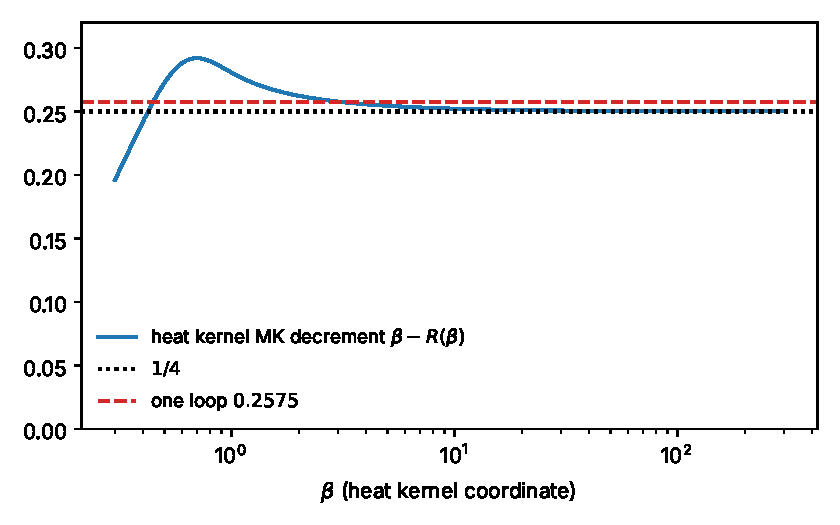
\includegraphics[width=0.85\textwidth]{figures/mk_cover.pdf}
\caption[The decrement $\beta-R(\beta)$ of the heat kernel projected Migdal Kadanoff map for SU(2)]{The decrement $\beta-R(\beta)$ of the heat kernel projected Migdal Kadanoff map for SU(2), computed in double precision on the grid of the covering computation. It is positive throughout, peaks near the crossover, and tends to $(1-b^{-2})\E S_{\mathrm{BPY}}=1/4$, slightly below the one loop value.}
\label{fig:coverB}
\end{figure}

The computed decrement lies in $[0.196,0.292]$ on the grid, with its maximum near $\beta\approx0.7$. Below $\beta=0.38$ we have $u_2<0.02$. We use this as the working definition of strong coupling for the ladder. We know no explicit convergence radius for a cluster expansion in these coordinates: the Osterwalder Seiler theorem gives an unspecified $\beta_0$ for the Wilson action, and after several steps the weight is a general class function, so we do not claim that the grid overlaps a region where the cluster expansion\index{cluster expansion} converges. Above $\beta=300$ the asymptotics of Remark~\ref{prop:decrementB}, with a positive $O(1/\beta)$ correction fitted at $0.021/\beta$, are a leading order derivation and a fit, not a bound. A computer assisted theorem on a grid would need interval arithmetic for $R$ at the grid points, interval arithmetic for the likelihood ratio inequality, and an explicit bound on the $O(1/\beta)$ remainder. Each is a finite computation with explicit, smooth functions, and none has been done here. The enclosures with an explicit rounding allowance are those of Chapter~\ref{ch:progress}.

\subsection{The correlation length as a first passage time}

Define the renormalization walk $\beta_{\ell+1}=R(\beta_\ell)$ of the projected map and its first passage time below the strong coupling threshold,
\[
J(\beta)=\min\{\ell:\beta_\ell<\beta_*\},\qquad\beta_*=0.38 .
\]
Each step multiplies the lattice spacing by $b$, so lengths measured in units of the original spacing are $b^{J}$ times lengths on the final lattice. If $\xi_*$ is the correlation length of the strong coupling theory reached after $J$ steps (at a coupling below $\beta_*$ that depends on $\beta$), and if the projected walk stands for the true recursion, then
\[
\xi(\beta)=b^{J(\beta)}\,\xi_* .
\]
The telescoping identity $\beta-\beta_J=\sum_{\ell<J}\delta(\beta_\ell)$, with $\delta(\beta)=\beta-R(\beta)$, is a deterministic form of Wald\index{Wald identity}'s identity:
\[
J(\beta)=\frac{\beta-\beta_J}{\bar\delta_J},
\]
where $\bar\delta_J$ is the average decrement along the path. If, as the leading order derivation of Remark~\ref{prop:decrementB} suggests, $\delta(\beta)=\delta_\infty+O(1/\beta)$ with $\delta_\infty=(1-b^{-2})\E S_{\mathrm{BPY}}$, the average converges and
\[
\log\xi(\beta)=\frac{\ln b}{(1-b^{-2})\E S_{\mathrm{BPY}}}\,\beta+O(\log\beta).
\]
This is the ladder's form of asymptotic freedom\index{asymptotic freedom}, with the coefficient written as a ratio of $\ln b$ to $(1-b^{-2})$ times the mean of a generalized gamma convolution\index{generalized gamma convolution}. In the Riemann programme~\cite{PS26a} we read the zeros through hitting times of a ladder in the abscissa; here the correlation length is a hitting time of a ladder in the coupling.

\subsection{The gap criterion}

\begin{proposition}[first passage criterion for the projected ladder]\label{prop:criterionB}
For the walk $\beta_{\ell+1}=R(\beta_\ell)$ of the heat kernel projected map, suppose that $R$ is continuous and that
\begin{enumerate}
\item[(A)] $\delta(\beta)>0$ for every $\beta>0$, and
\item[(B)] $\delta(\beta)\to\delta_\infty>0$ with $O(1/\beta)$ corrections.
\end{enumerate}
Then every coupling reaches the strong coupling region $\beta<\beta_*$ in $J(\beta)=\beta/\delta_\infty+O(\log\beta)$ steps.
\end{proposition}

\begin{proof}
Condition (A), with continuity and the asymptotics (B), bounds $\delta$ below by a positive constant on $[\beta_*,\infty)$, so $J(\beta)<\infty$ and the estimate on $J$ follows by summing.
\end{proof}

The proposition is about the projected map and says nothing yet about a gap. To reach the gap on the Migdal Kadanoff hierarchical lattice, at least three further things are needed, and none is proved here.

\begin{remark}[what the criterion would give for the gap]
Suppose in addition that (C) the exact recursion on the hierarchical lattice is described by the projected map, so that the steps above are steps of the true flow; (D) the theories reached after $J(\beta)$ steps, which sit at couplings below $\beta_*$ that vary with $\beta$, have a positive lattice mass bounded below by a constant $m_*$ uniformly in $\beta$, which is a cluster expansion statement with explicit constants; and (E) in physical units, where $a(\beta)$ is the physical lattice spacing of the real theory, $a(\beta)\Lambda\propto\exp(-3\pi^2\beta/11)$ at one loop times a power of $\beta$ from the two loop term, the product $a(\beta)\,b^{J(\beta)}$ is bounded as $\beta\to\infty$. Then the correlation length of the hierarchical lattice theory is at most $b^{J(\beta)}/m_*$ in lattice units, hence bounded in physical units. That is a bound on a correlation length. It is not the uniform Thorin gap inequality: the hierarchical lattice has no spectral measures (see the end of this remark), and Theorem~\ref{thm:equivB} would need in addition nonnegative measures $\mu^{(a)}$ with $\sup_a\int e^{-\alpha_0E}\,d\mu^{(a)}$ finite and uniformity in the volume, which are the two missing steps recorded after the Osterwalder and Seiler theorem above. The status of the three conditions is as follows. (C) is open: the exact recursion acts on all character coefficients, and the agreement of the two is numerical only ($0.012$ over eight steps). (D) is open: no explicit convergence radius is known to us, nor a lower bound on the mass uniform on $(0,\beta_*]$. (E) is not merely open: as stated it fails for the ladder with $\delta_\infty=\frac14$ ($b=2$): $b^{J(\beta)}$ grows like $\exp(4\ln2\,\beta)=\exp(2.773\,\beta)$ while the one loop $a(\beta)$ decays like $\exp(-2.692\,\beta)$, so the product grows like $\exp(0.081\,\beta)$ times a power, because the Migdal Kadanoff decrement differs from the one loop value $0.2575$ (Remark~\ref{prop:decrementB}). Only with the ladder's own scale $a_{\mathrm{lad}}(\beta)=b^{-J(\beta)}$ is (E) close to the definition of $J$, and then no two loop term enters. So the conclusion of this remark is conditional on a scale matching that the ladder does not supply. If $\delta(\beta)=\delta_\infty+c/\beta$ then summing gives $J(\beta)\approx\beta/\delta_\infty-(c/\delta_\infty^2)\ln\beta$, so the sign and size of the logarithmic term, set against the power of $\beta$ in $a(\beta)$, would decide whether the product is bounded if the exponential rates agreed. Lemma~\ref{lem:posB} gives reflection positivity of the $\Z^4$ theory whose plaquette weight is a given rung. It does not give reflection positivity, a transfer matrix or spectral measures for the hierarchical lattice, so the Thorin densities of the hierarchical flow are not defined by it.
\end{remark}

Condition (B) is the leading order derivation of Remark~\ref{prop:decrementB}, with the remainder not bounded. Condition (A) for the projected ladder at every coupling is Corollary~\ref{cor:contracts}, which proves $R(\beta)<\beta$; Remark~\ref{prop:coverB} records the floating point evidence on $[0.3,300]$ that preceded it. So for the projected ladder, granted the continuity of $R$, the first passage time is finite at every coupling, and the linear growth of $J$ rests on (B). Confinement itself on the hierarchical lattice is Ito\index{Ito, K. R.}'s 1985 theorem; the criterion above is a statement about the projected map only. What remains is the relation between the projected map and the exact recursion, the relation between the approximation and the real theory, and the strong coupling mass with explicit constants, which are the subjects of Chapters~\ref{ch:path} and~\ref{ch:sandwich}.

\section*{Exercises}
Exercises 1 to 3 refer to Section~\ref{ch:latticemc}, 4 to 7 to Section~\ref{ch:mk}, and 8 to 11 to Section~\ref{ch:verification}.
\begin{enumerate}
\item Show that overrelaxation preserves the action and leaves the Haar measure invariant.
\item Show that the generalised eigenvalue problem recovers the lowest masses exactly when the number of states contributing to the correlator equals the size of the matrix.
\item Explain why the variance of a glueball correlator approaches a constant at large $\tau$.
\item Derive the general formula $1/t''=b^{d-4}/t-(b^{d-2}-1)\E S_{\mathrm{BPY}}/(2b^2)$ in detail, and discuss the cases $d=2$ and $d=3$.
\item Verify the identity $\sum_{i<j}(\theta_i-\theta_j)^2=N\sum_i\theta_i^2$ when $\sum_i\theta_i=0$.
\item Show that for SU(2), $\chi_2(\theta)/2=\cos\theta$, and hence that $u_2=\E[\cos\theta]$ under the normalised plaquette law.
\item Compute the ratio $\pi^2(1-b^{-2})/(11\ln b)$ for $b=2,3,4$ and explain why the Migdal Kadanoff coefficient depends on $b$.
\item Show that if $R$ is increasing and $R(\beta_{i+1})<\beta_i$ for consecutive grid points, then $R(\beta)<\beta$ on the whole interval, and explain why a floating point check of the grid inequality is not an enclosure.
\item Using the image sum, prove the likelihood ratio property of the SU(2) heat kernel for all sufficiently small $t$.
\item Estimate the number of Migdal Kadanoff steps from $\beta=10$ to strong coupling using only the asymptotic decrement, and compare with the table of doublings in Section~\ref{ch:mk}, interpolating between $\beta=8$ and $\beta=16$.
\item Explain why projecting onto the heat kernel family after each step, rather than following all character coefficients, changes the trajectory by only a small amount at weak coupling.
\end{enumerate}
